\section{Theoretical Results} \label{sec:theory}

We theoretically analyze the quality of weak supervision's label model, taking into account the impact of misspecification when using weakly labeled versus fully labeled data. %The results produce a practical criterion for valuing supervision. %First, we discuss the error in the labeling functions' accuracy parameters $a_i$ for both the labeled and unlabeled data case. 
%Then, we propagate this error into our computation of the 
In \ref{subsec:decomp} we give 
%bounds the accuracy estimation error that arises from using unlabeled data under misspecification. Next, we use these to present
an exact decomposition of the generalization error of the label model, which demonstrates how misspecification is present in both the learning and aggregation steps of the model when data is weakly labeled and only present in the latter when data is fully labeled. In \ref{subsec:scaling}, we bound the generalization error using this framework to show how the weakly labeled case has an additional standing bias of $\mathcal{O}(d/m)$. Given this standing bias, in \ref{sec:misspec}, we introduce a simple method that under certain conditions can correct for dependency-based misspecification. We then analyze this correction's impact on generalization error. 



% misspecification impacts parameter estimation only when the data is unlabeled; therefore, this particular term is crucial in determining which dataset has lower generalization error. We then discuss ways to mitigate misspecification's impact on parameter estimation. Lastly, using our error analysis we propose our data value criterion for choosing between and combining unlabeled and labeled data.
%and present upper and lower bounds on the generalization error of our label model, again for both labeled and unlabeled data cases separately. In each part, we contrast the labeled and unlabeled data settings. Lastly, we use these bounds to propose a data value criterion.

\subsection{Decomposition Framework}
\label{subsec:decomp}%for WS Label Model}

%We define the generalization error as $\mathbb{E}[l(\widetilde{Y}, Y)]$, where 
%\begin{align*}
%&l(\widetilde{y}_i, y_i) = -\left(\frac{1 + y_i}{2}\right) \log \widetilde{\Pr}(Y = 1 | \lf = \lf(x_i)) \\
%&- \left(\frac{1 - y_i}{2}\right) \log \widetilde{\Pr}(Y = -1 | \lf = \lf(x_i))
%\end{align*} is the cross-entropy loss on a point $(x_i, y_i)$. The expectation is taken over $(Y, \bm{\lf})$, the random triplets chosen to estimate each $a_i$, and the finite samples used. 

%One immediate consequence of model misspecification in the case of unlabeled data is that the  $\lf_i, \lf_j, \lf_k$ used to estimate $a_i$ may not be pairwise conditionally independent. This results in biased (and inconsistent) estimation when data is unlabeled. In contrast, in the labeled data setting, the $a_i$'s can be directly estimated as $\Ehat{\lf_i Y}$.

%\begin{lemma}[Accuracy Bias] 
%Suppose each $a_i$ is estimated by randomly choosing $\lf_j$ and $\lf_k$ in \eqref{eq:triplet} in the case of unlabeled data, and let $a_{\min} = \min_i a_i$ and $b_{\min} = \min_{i, j} \E{}{\lf_i \lf_j}$. Assume that the true distribution satisfies \eqref{eq:true_pgm} with $|E_{\lf}| = d$ and that $a_{\min} b_{\min} \ge \frac{d - 1}{m - 2}$. Then the expectation of the asymptotic bias of $\widetilde{a}^U$, which we refer to as $\bar{a}$, is 
%\begin{align}
%     \frac{d \varepsilon_{\min}}{m - 1} \left( \frac{(m - 2d) b_{\min}^2}{m - 2} \right)\le  \|\E{}{\widetilde{a}^U} - a\|_1 \le \frac{d \varepsilon_{\max}}{m - 1} \left(\frac{2}{b_{\min} a_{\min}} + \frac{1}{b_{\min}^2 a_{\min}^2} \right),
%\end{align}

%$\varepsilon_{\max}$ is an upper bound on $\varepsilon_{ij} = \E{}{\lf_i \lf_j} - \E{}{\lf_i Y} \E{}{\lf_j Y}$ for all $(i, j) \in E_{\lf}$, and $\varepsilon_{\min} \ge 0$ is a lower bound. In particular, $\varepsilon_{ij} = \frac{8}{Z_{ij}} \sinh(\theta_{ij})(\cosh(2\theta_i) + \cosh(2\theta_j) - \frac{64}{Z_{ij}^2} \sinh^2(\theta_{ij}) \sinh(2\theta_i) \sinh(2\theta_j)$ where $Z_{ij}$ is a product of marginal cumulant functions.  
%\label{lemma:accuracy_bias}
%\end{lemma}

%From this result, we see that when $d = 0$, $\E{}{\widetilde{a}^U} = \E{}{\widetilde{a}^L} = a$, meaning that the asymptotic estimator is unbiased. However, as the number of dependencies or the strength of the correlation $\theta_{ij}$ relative to $\theta_i$ and $\theta_j$ increases, there is a standing bias, and it worsens. \todo{where should I put assumptions used for these theorems? i.e. $\theta_i, \theta_j, \theta_{ij} \ge 0$ for this analysis}

%\paragraph{Bounding the generalization error}

%The estimation error for $\widetilde{a}_i^U$ is now propagated into the generalization error for the label model. We define the generalization error as $\mathbb{E}[l(\widetilde{Y}, Y)]$, where \[l(\widetilde{y}_i, y_i) = -\left(\frac{1 + y_i}{2}\right) \log \widetilde{\Pr}(Y = 1 | \lf = \lf(x_i)) - \left(\frac{1 - y_i}{2}\right) \log \widetilde{\Pr}(Y = -1 | \lf = \lf(x_i))\] is the cross-entropy loss. The expectation is taken over $(Y, \bm{\lf})$, the random triplets chosen to estimate each $a_i$, and the finite samples used. 

We present our first result, a decomposition of weak supervision's generalization error into four components. The last two components, the inference bias and parameter estimation error, reflect the role of misspecification.
\begin{theorem}
The generalization error has the following decomposition:
\begin{align}
    &\E{}{l(\widetilde{Y}, Y)} = \underbrace{H(Y | \bm{\lf})}_{\mathclap{\mathrm{Irreducible \; error}}} - \underbrace{\E{\N}{\KL(\Pr(\bm{\lf}) || \hat{\Pr}(\bm{\lf}))}}_{\mathrm{Observable \; sampling \; noise}} + \nonumber \\ %\E{}{\frac{1 + a}{2} \log \frac{1 + \widetilde{a}}{1 + a}  + \frac{1 - a}{2} \log \frac{1 - \widetilde{a}}{1 - a} } - \nonumber \label{eq:decomposition} \\
    &\sum_{\mathclap{(i, j) \in E_{\lf}}} \;\;\; \underbrace{I(\lf_i; \lf_j | Y)}_{\mathrm{Inference \; bias}} +  \sum_{i = 1}^m \underbrace{\E{Y, \N, \tau}{\KL(\mathrm{Pr}_{\lf_i | Y} || \widetilde{\Pr}_{\lf_i | Y })}}_{\mathrm{Parameter \;estimation \;error}} \nonumber,
\end{align}

where $I(\lf_i; \lf_j | Y)$ is the conditional mutual information between labeling functions that share an edge and $H(Y|\bm{\lf})$ is conditional entropy. $\Pr$ refers to the true data distribution, while $\hat{\mathrm{Pr}}$ and $\widetilde{\mathrm{Pr}}$ refer to the estimated probabilities in \eqref{eq:inference}.

\label{thm:decomposition}
\end{theorem}

We now discuss the significance of each term in this decomposition. The first two terms are independent of misspecification and are present in both the weakly and fully labeled cases:
\begin{itemize}
    \item Irreducible error: this term is an intrinsic property of the distribution of $(Y, \bm{\lf})$ and is always present in bias-variance decomposition. Here, it roughly measures the quality of the labeling functions.
    \item %\steve{I'm confused by the negative sign in front of this term.} 
    Observable sampling noise: particular to our inference approach, this term is the expected Kullback-Leibler divergence between the true marginal distribution of the observable labeling functions and the empirical distribution. It is a common notion of sampling noise~\citep{domingos2000unified, yang2020rethinking} and approaches $0$ asymptotically.
\end{itemize}

For the last two terms, misspecification plays a different role depending on the data type. 
\begin{itemize}
    \item Inference bias: this term is the conditional mutual information between conditionally dependent labeling functions. Particular to our inference approach, it describes the approximation error of using marginal probabilities of singletons rather than their product distributions. Therefore, it represents the role of misspecification at the aggregation step in \eqref{eq:inference} and is present for both data types. It is independent of parameter estimation method.
    \item Parameter estimation error: this term describes the difference between the true distribution of $\lf_i$ conditional on $Y$ versus the estimated distribution. As discussed in section \ref{sec:background}, this directly depends on accuracy parameter estimation approach for $\widetilde{a}_i$. In the labeled data case, we know that this error corresponds to sampling noise and thus asymptotically approaches $0$. For the weakly labeled case, in addition to sampling noise the estimator in \eqref{eq:triplet} is also biased, as are many method-of-moments approaches. Furthermore, misspecification impacts the learning step of the WS label model and makes the estimator inconsistent when $\lf_i, \lf_j,$ and $\lf_k$ used to produce $\widetilde{a}_i^U$ are not pairwise conditionally independent.
\end{itemize}

We now discuss in detail the scaling of these last two terms, which highlights the tradeoff between labeled and weakly labeled data under misspecification.


%We now examine the role of misspecification in these bounds. The decomposition of the generalization error in \eqref{eq:decomposition} isolates the accuracy parameters in the first term, where $a_i$ is the true accuracy and $\widetilde{a}_i$ is the estimated accuracy. In the case of unlabeled data, $\widetilde{a}_i$ is always a biased estimator as suggested by \eqref{eq:triplet} with bias $\mathcal{O}(1/\sqrt{n})$. However, it is also inconsistent due to misspecification with additional error $\mathcal{O}(d/m)$, since the $\lf_i, \lf_j, \lf_k$ used to estimate $a_i$ may not be pairwise conditionally independent. On the other hand, when we have labeled data, accuracies are observable and thus the only difference between $a_i$ and $\widetilde{a}_i$ is due to sample noise---misspecification has no impact.

%The remaining terms in \eqref{eq:decomposition} are the same for both labeled and unlabeled data. The conditional entropy $H(Y | \bm{\lf})$ is the irreducible error, and the expected KL-divergence $\E{}{D_{KL}(\Pr(\bm{\lf}) || \hat{\Pr}(\bm{\lf}))}$ is a form of variance caused by using the empirical pdf for the observable labeling functions. Lastly, However, since this term is the same for both the labeled and unlabeled data settings, it does not play a role in choosing between them using the data value criterion; the only place where misspecification matters in the criterion is the accuracy error $\mathcal{O}(\frac{d}{m})$.

\subsection{Scaling of the Generalization Error} %under Misspecification}
\label{subsec:scaling}

Using our framework presented in Theorem \ref{thm:decomposition}, we bound individual terms to understand the scaling of the error due to misspecification in both the weakly labeled and fully labeled cases. Since the irreducible error is always present regardless of our approach or setting, we focus on bounding the \textit{excess generalization error}, defined as $R^{\mathrm{excess}}_L = R_L -  H(Y|\bm{\lf})$ for labeled data and similarly $R^{\mathrm{excess}}_U$ for unlabeled data.  We use $\B_I = \sum_{(i, j) \in E_{\lf}} I(\lf_i; \lf_j | Y)$ as a placeholder for the inference bias in these bounds since it is independent of our two settings, and while it does scale in $d$, it is simply a measurement over the true data distribution. We present upper bounds here and a lower asymptotic bound in the Appendix.

We first present an upper bound on the excess generalization error in the labeled data case. 
\begin{theorem}
Suppose that there are $|E_{\lf}| = d$ dependencies. When we perform weak supervision as described in section \ref{sec:background} using $n_L$ labeled samples and a misspecified model,
%\bcw{Shouldn't $\varepsilon_{\max}$ appear in this expression somewhere?}
\begin{align}
   R_L^{\mathrm{excess}} \le \frac{m}{2n_L} + \B_I + o(1/n_L) 
\end{align}
\label{thm:labeled}
\end{theorem}

%\steve{what about the ``observable sampling noise''?} 
In this labeled data bound, $\frac{m}{2n_L}$ is an upper bound on the parameter estimation error and solely represents the sampling noise of $\widetilde{a}_i^L = \Ehat{\lf_i Y}$, which asymptotically approaches $0$. %$d\log 2$ is a simple upper bound on the inference bias that is obtained by definition of the mutual information. 
Therefore, the only standing bias is $\B_I$ due to inference approach. On the other hand, when there is no model misspecification, the excess error is $\mathcal{O}(1/n_L)$, and thus for large $n_L$ our label model would approach the true distribution of $\Pr(Y | \bm{\lf})$.  

We next present an upper bound on the excess generalization error in the weakly labeled case. Define $\varepsilon_{ij} = \E{}{\lf_i \lf_j} - \E{}{\lf_i Y} \E{}{\lf_j Y}$ as the extent of misspecification on a single pair of labeling functions, and let $0 \le \varepsilon_{\min} \le \varepsilon_{ij} \le \varepsilon_{\max}$ for all pairs $(i, j)$ under our assumptions on the graphical model in section \ref{sec:background}. We give the exact value of $\varepsilon_{ij}$ in terms of canonical parameters 
%\steve{I'm confused. I haven't read the appendix, but didn't you just define $\varepsilon_{ij}$ in this paragraph?} 
in the Appendix. 
%be bounds on the value of $\E{}{\lf_i \lf_j} - \E{}{\lf_i Y} \E{}{\lf_j Y}$ over all pairs $(\lf_i, \lf_j)$ in terms of the canonical parameters $\Theta$. Then,
\begin{theorem}
Suppose that there are $|E_{\lf}| = d$ dependencies. When we perform weak supervision as described in section \ref{sec:background} using $n_U$ weakly labeled samples and a misspecified model, 
\begin{align}
    R_U^{\mathrm{excess}} \le  & \varepsilon_{\max} \left(\frac{c_1 d}{m} + \frac{c_2}{\sqrt{n_U}} + \frac{c_3d }{m n_U}\right) \\
    + &\frac{c_4 m}{n_U} + \B_I + o(1/n_U), \nonumber
\end{align}
where $c_1, c_2, c_3,$ and $c_4$ are constants that depend on the intrinsic quality and correlations of the labeling functions, all defined in the Appendix. 
\label{thm:unlabeled}
\end{theorem}

In this weakly labeled data bound, we again have an observable sampling noise term $\frac{c_4 m}{n_U}$, where the difference in the constant term comes from estimating terms of the form $\Ehat{\lf_i \lf_j}$ in \eqref{eq:triplet} rather than $\Ehat{\lf_i Y}$ in the labeled data case. However, for this case the parameter estimation error has an additional misspecification term $\B_{\mathrm{est}} :=\varepsilon_{\max} \left(\frac{c_1 d}{m} + \frac{c_2 }{\sqrt{n_U}} + \frac{c_3 d}{m n_U}\right)$ which depends on both the extent and amount of misspecification. Therefore, asymptotically the weakly labeled case has a standing bias bounded by $\frac{c_1 d \varepsilon_{\max}}{m} +\B_I$ in comparison to the labeled case's $\B_I$, and the finite sample regime contributes additional sampling noise for the weakly labeled case that scales in $\varepsilon_{\max}$. In the case of no misspecification $(d = 0, \varepsilon_{\max} = 0)$, the only term still present is $\frac{c_4 m}{n_U}$, so our label model would also approach the true distribution of $\Pr(Y | \bm{\lf})$ but at a different rate. 

\paragraph{Partial Recovery} Our result holds almost exactly for the partial recovery case, where there are $d$ dependencies and we have recovered a subset $d'$ of them via structure learning or some other approach. In particular, the additional estimation error is now scales at rate $\frac{(d - d') \varepsilon_{\max}  }{m - 2d'}$. \mayee{double check}
%comparison of the weakly labeled versus fully labeled case reduces to the sampling noise of \eqref{eq:triplet} versus directly estimating $\E{}{\lf_i Y}$, namely $\frac{c_4 m}{n_U}$ versus $\frac{m}{2n_L}$ where the only difference is the constant factor. 
%The result follows from tracing error through two steps, (i) accuracy estimation from Lemma \ref{lemma:accuracy_bias}, and (ii) inference using the learned label model. The accuracy estimation step involves sampling error of order $\frac{m}{n}$ for both the labeled and unlabeled cases, although the size of the datasets $n_U$ versus $n_L$ is important here. However, for the unlabeled case there is an additional $\frac{m}{\sqrt{n}}$ that comes from the fact that the triplet method is biased and another $m\log (1 + d\varepsilon_{\max} /m^2)$ due to the extra parameter error from Lemma \ref{lemma:accuracy_bias} caused by misspecification. The second step is identical for both cases; since dependencies are assumed to be unknown, the inference is approximate, and we compute the error to be of order $d \log (1 + \varepsilon_{\max})$.

%The error bounds for unlabeled versus labeled data also suggests a tradeoff among the $d$ dependencies, $n_U$, and $n_L$. When $d$ is small and $\varepsilon_{\max}$ is small (i.e. dependencies among labeling functions are few and weak), then $\log(1 + d \varepsilon_{\max} / m^2) \approx d \varepsilon_{\max} / m^2$, and thus the error from estimating accuracies is of order $d \epsilon_{\max} / m$. Therefore, when $n_L \ll n_U$, a model learned using unlabeled data \emph{can still perform better than one with labeled data, even under misspecification}. On the other hand, if there are many strong dependencies that weren't modeled, the accuracy parameters are too biased such that using a small amount of labeled data is still better. This tradeoff suggests a useful way for practitioners to assign value to labeled versus unlabeled data; we discuss our proposed data value criterion below.



%The model misspecification plays a role in this error for both the unlabeled data and labeled data settings, since the true distribution cannot be factorized according to \eqref{eq:inference} but rather has conditional probabilities on pairs of labeling functions, namely $\Pr(\lf_i, \lf_j = \lf_i(X), \lf_j(X) | Y = 1)$ for each $(i, j) \in E_{\lf}$.

\subsection{Correcting for misspecification}\label{sec:misspec}

How can we reduce the penalty for dealing with such unrecovered dependencies? This is a common problem in method-of-moments approaches to latent variable estimation beyond WS~\citep{anandkumar12, chaganty2014estimating}---in particular, multi-view learning---where most literature assumes the dependencies are known or that the true data distribution exhibits conditional independence among all observable variables. We examine how to reduce misspecification for our particular method described in \eqref{eq:triplet}, but we also discuss how our correction can be applied to other algorithms in the Appendix to show its use extended to other weak supervision approaches and more general latent variable estimation problems.

%Note that this correction for misspecification is applicable to many method-of-moments approaches beyond its use in WS, such as \cite{anandkumar12, chaganty14}, in order to more generally learn parameters of latent variable models. 

In our parameter estimation approach, if there exists an $\lf_i$ such that there are no $\lf_i, \lf_k$ where all three labeling functions are pairwise conditionally independent given $Y$, then it is not possible to learn  $a_i$. In less demanding cases, %the natural approach is to learn these dependencies via \emph{structure learning}. This can be done in the unlabeled data setting \citep{bach2017learning, varma2019learning}. However, it may involve solving a challenging optimization problem (e.g., an SDP). 
we suggest an alternative approach based on \emph{medians}. Note that the contribution to the accuracy estimation error coming from misspecification is due to randomly selecting triplets that violate pairwise conditional independence, which occurs with probability $O(d/m^2)$, 
in our average $\widetilde{a}_i^U$. To reduce this impact, we estimate each $a_i$ by computing the median accuracy over all pairs $\lf_j, \lf_k$ using \eqref{eq:triplet} a total of ${m - 1 \choose 2}$ times.
\begin{proposition}
%Denote $\widetilde{a}_i^{(j, k)}$ as the estimate in \eqref{eq:triplet}. 
Define $\widetilde{a}_i^M = \mathrm{median}(\{\widetilde{a}_i^{(j, k)} \; \forall \; j, k \neq i \})$. Then $\widetilde{a}_i^M$ is not affected by misspecification and is thus a consistent estimator if $m > 5$, $d < \frac{(m - 1)(m - 2)}{4}$, and $n_U \ge n_0$, where $n_0$ is $\omega(1/\varepsilon_{\min}^2)$.

Refer to $\rho_{n_U} = \max_i \E{}{(\widetilde{a}_i^M - a_i)^2}$ as the rate of convergence for $\widetilde{a}^M$. Under these conditions, the excess generalization error from using $n_U$ weakly labeled samples and a corrected model is, for constant $c_\rho$,
\begin{align}
    R_C^{\mathrm{excess}} \le c_\rho m  \rho_{n_U} + \B_I + o(1/n_U)
\end{align}
\label{prop:medians}
\end{proposition}

Note that while we assume sparsity of $E_{\lf}$ for simpler analysis in section \ref{sec:theory}, the conditions above on $d$ and $m$ apply for any given dependency graph in the WS setting. While $\rho$ can be analyzed in detail as a variant of the medians-of-means estimator, we emphasize that $\lim_{n_U \rightarrow \infty} \rho(n_U) = 0$, and thus the standing bias of order $\mathcal{O}(d/m)$ due to misspecification has been eliminated. This reduction in generalization error has significant implications for the value of labeled versus weakly labeled data in corrected settings. %We verify this improvement in generalization error in section \ref{sec:exp}. 

%Finally, this median-based approach applies to other steps of the label model. A similar technique, where we partition the sources into $q$ groups, perform inference separately with each group to get $\widetilde{Y}$, and take the median, can be used to reduce the impact of misspecification in the approximate inference step.

%This reduces the probability of selecting an unbiased triplet (as the median) to $O(1-(d/m^2)^{t+1})$. This technique helps us in cases where $d = o(m^2)$. 

\subsection{Synthetic Experiments}

We validate the fundamental principles of our theoretical framework using synthetic data. We measure the excess generalization error vs. $\log(n)$ in the well-specified, misspecified and corrected settings on synthetic data with $m=10$ labeling functions, accuracies drawn uniformly from $[.55, .75]$ and extents of misspecification fixed at $\varepsilon=0.1$. A more detailed protocol for synthetic experiments is available in the \todo{Appendix}.
%First, in the labeled and unlabeled settings, a well-specified model achieves an asymptotic error of zero. Under misspecification, we see the presence of $\B_I$ in both settings, and an additional parameter estimation bias $\B_{\mathrm{est}}$ in the unlabeled setting. Finally, we expect a corrected model to mitigate this parameter estimation bias. 
%We report how our empirical results match up with theory in \autoref{fig:gen_err}. 
Our results are in \autoref{fig:gen_err}. With no misspecification ($d=0$) the labeled and unlabeled estimators both tend towards zero. Under misspecification ($d=5$), we see that learning from unlabeled data results in an additional standing bias that parallels $\B_{\mathrm{est}}$. Median aggregation reduces this bias and results in error converging to roughly similar values, paralleling $\B_I$, in both the weakly-labeled and labeled cases.

%%%% UNCOMMENT
% \begin{figure}
%     \centering
%     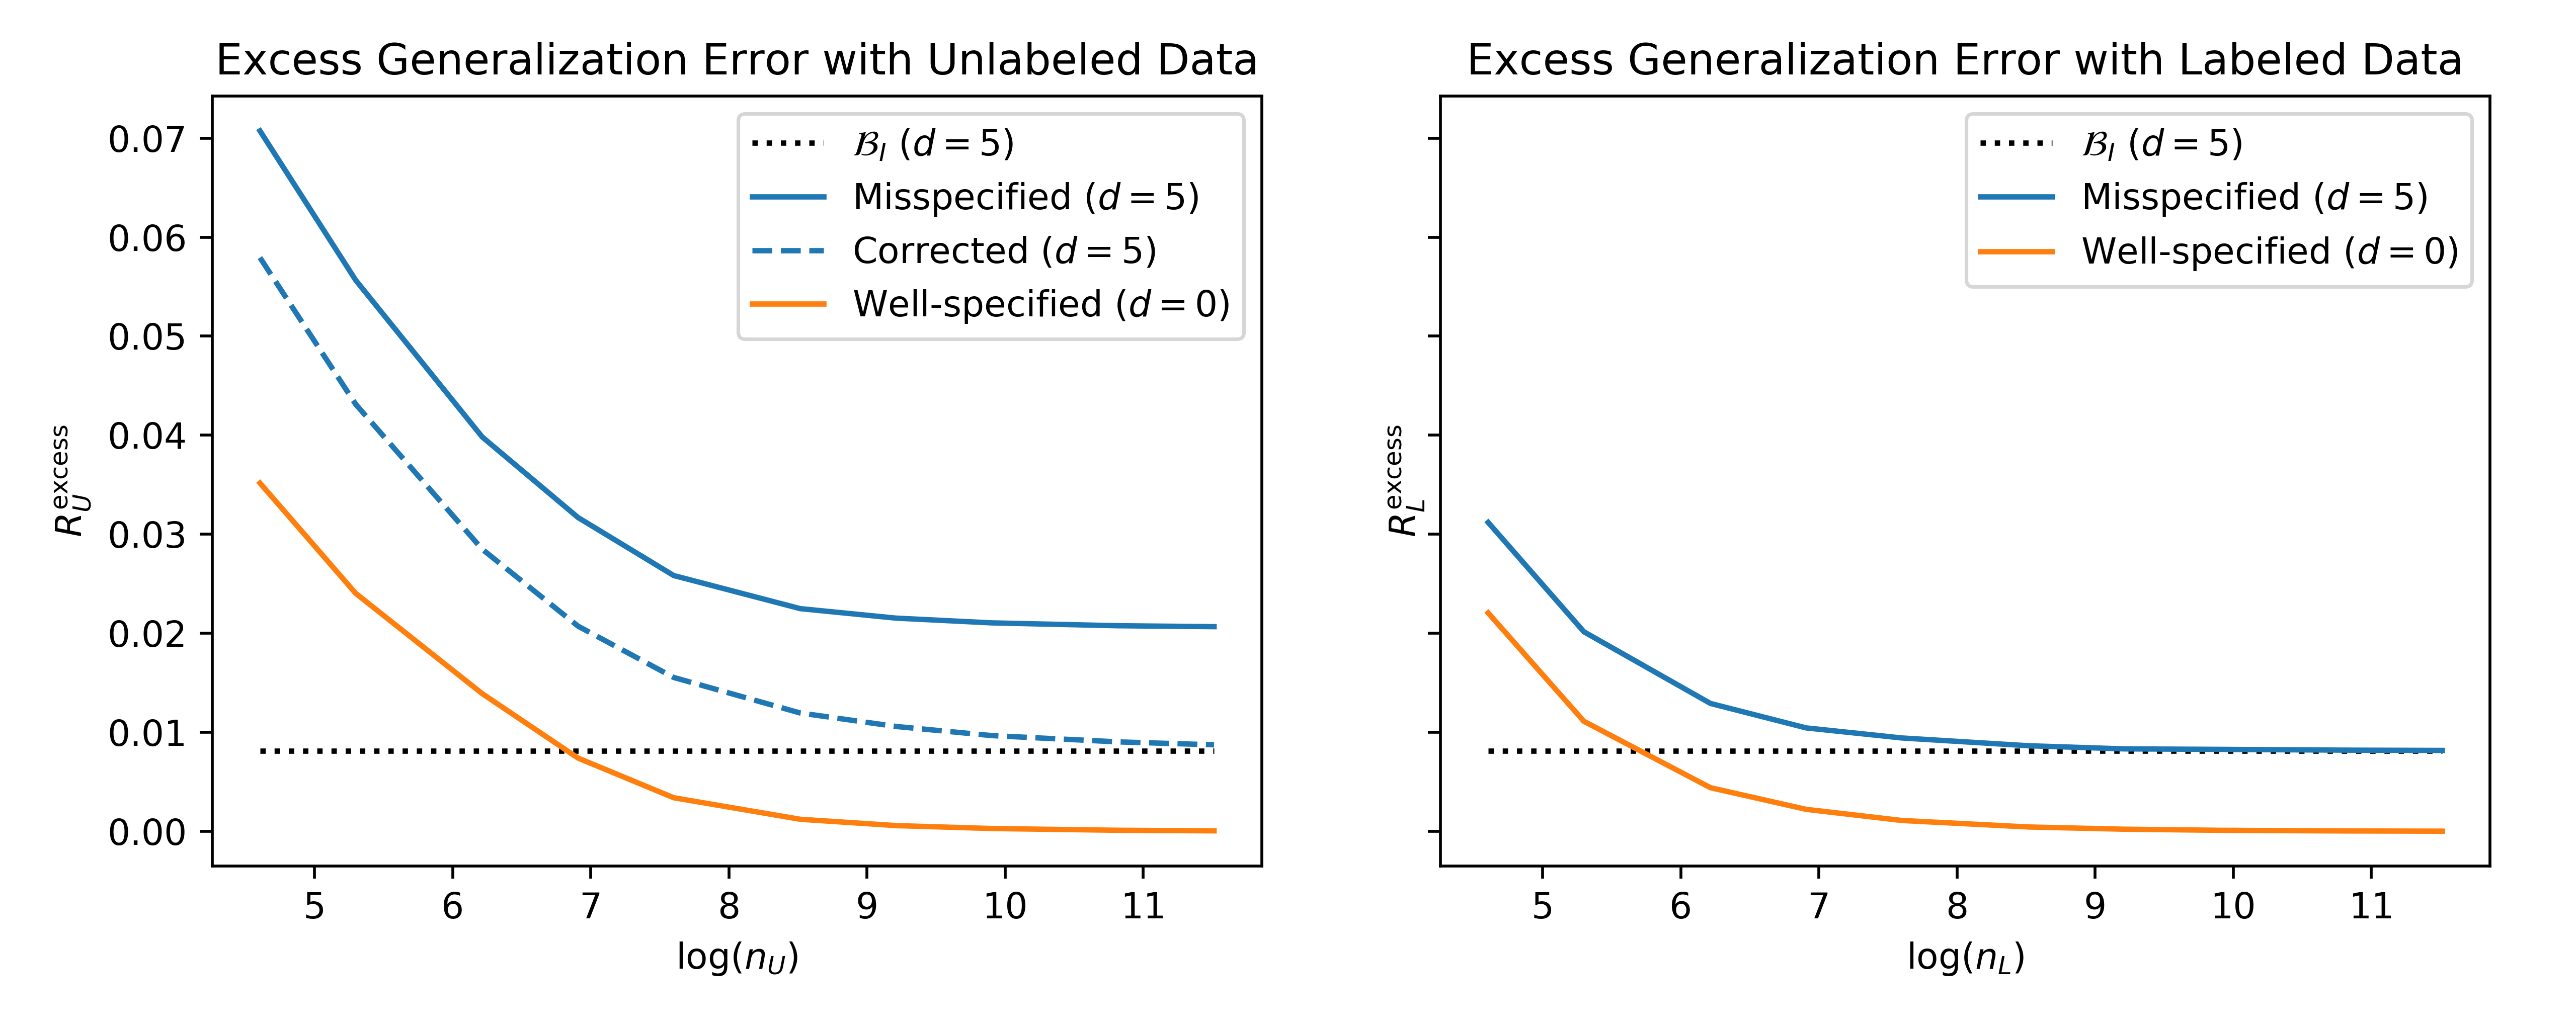
\includegraphics[width=.48\textwidth]{figures/biases.png}
%     %
%     \caption{Excess generalization error vs. $\log(n)$ with different estimators for synthetic data. Left: comparison of unlabeled data performance under the three discussed settings. Right: comparison of labeled data performance for well-specified and misspecified models. A dashed line repesenting an empirical ``$\B_I$'' suggests how inference bias is present in both data cases.  % With no misspecification ($d=0$) the labeled and unlabeled estimators both converge to an asymptotic error of zero. Under misspecification ($d=5$), we see that learning from unlabeled data results in an additional $\B_{\mathrm{est}}$ standing bias due to misspecification, and median aggregation corrects for this bias so that error converges to $\B_I$.
%     }
%     \label{fig:gen_err}
% \end{figure}